
%------------------------------------------------

\section{Random variables and probability distributions}\index{random variable}\index{probability distribution}
\label{sec:rand_var}

\newthought{A random event} is an event that has more than one possible outcome, to which a probability may be associated.

The outcome of a random event is not known, only the probabilities of the possible outcomes are known.

We can associate a random variable $x$ to a random event $\mathbf{X}$.

The possible numerical values $x_{1}, x_{2}, \cdots$ corresponding to the possible outcomes are the probabilities $P(x_{1}), P(x_{2}), \cdots$, which forms a “probability distribution”\index{probability distribution}, obeying to the normalization condition (\ref{eq:norm_cond}).

\marginnote{ $ \sum_{i} P(n_{i}) = 1$ (\ref{eq:norm_cond})}

\begin{itemize}[$\to$]
	\item A set of $N$ observations of the random variable $x$ can be considered as a single observation of a vector $\vec{x} := (x_{1}, \cdots, x_{n})$.
	\item This is the definition of a histogram.
		\marginnote{What if a random variable covers a continuous interval?}
\end{itemize}

\subsection{Probability density function	}\index{probability density function}
\label{subsec:pdf}

Consider a sample space $\Omega \subset \mathbb{R}^{n}$.

A random extraction (experiment) will lead to an outcome (measurement) corresponding to one point $\vec{x} \in \Omega$.

We can associate a “probability density” $f(\vec{x})$ to any point $\vec{x} \in \Omega$, with $f(\vec{x}) \geq 0$.

The probability of an event $A$ is: 

\begin{equation}\label{eq:prob_event}
	P(A) = \int_{A} {f(\vec{x})} \,\mathrm{d}\vec{x}
\end{equation}

$f(\vec{x})$ is the differential probability, \ie the infinitesimal probability $\mathrm{d}P$ corresponding to the infinitesimal hyper-volume $\mathrm{d}\vec{x}$.

\begin{equation}\label{eq:differential_prob}
	f(\vec{x}) = \frac{\mathrm{d}P(\vec{x})}{\mathrm{d}\vec{x}}
\end{equation}

$f(\vec{x})$ obeys the normalization condition:

\begin{equation}\label{eq:differential_norm_cond}
	\int_{\Omega} {f(\vec{x})} \,\mathrm{d}\vec{x} = 1
\end{equation}

If $x$ is a 1-dim discrete variable:

\begin{equation}\label{eq:discrete_differential_prob}
	f(x) = \sum_{i = 1}^{n}{P_{i} \delta(x - x_{i})}
\end{equation}

In fact:

\begin{equation}
	\int_{-\infty}^\infty f(x) \,\mathrm{d}x = \sum_{i = 1}^{n}{P_{i} \int_{-\infty}^\infty \delta(x - x_{i}) \,\mathrm{d}x} = \sum_{i} P_{i} = 1
\end{equation}

If a variable is continuous, but we measure it with a discretized device, we can instead do:

\marginnote{This is the case of a measurement done with a MCA.

This is the case of a measurement of a particle track with a pixelated detector with pixel size $\delta x$.}

\begin{equation}
	P_{i} = \int_{x_{i}}^{x_{i} + \delta x} f(x) \,\mathrm{d}x
\end{equation}

\subsection{Cumulative distribution}\index{cumulative distribution}
\label{subsec:cdf}

\marginnote[6pt]{Monotonous increasing function from 0 to 1.}

It is defined as (\ref{eq:cumulative_distr}):

\begin{equation}\label{eq:cumulative_distr}
	F(x) = \int_{-\infty}^{x} f(y) \,\mathrm{d}y
\end{equation}

\begin{equation}
	F(\tilde{x}) = P(x \leq \tilde{x}) \,\forall \tilde{x}
\end{equation}

An example plot is (Figure~\ref{fig:CDF_PDF_Gaussian}):

\begin{figure}
	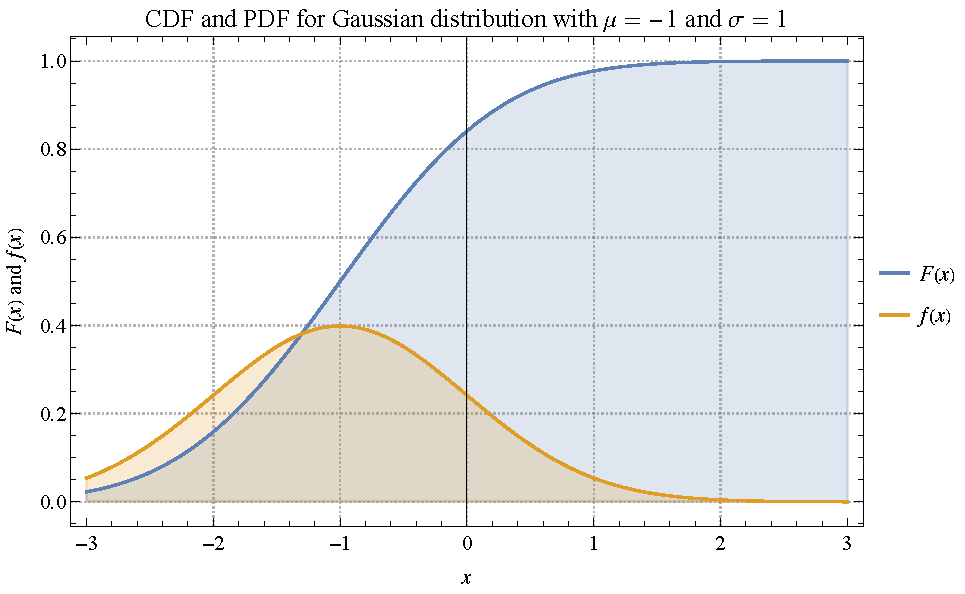
\includegraphics{probability/CDF_PDF_Gaussian.pdf}
	\caption[CDF and PDF for Gaussian distribution.][6pt]{CDF and PDF for Gaussian distribution with $\mu = -1$ and $\sigma = 1$.}
	\label{fig:CDF_PDF_Gaussian}
\end{figure}

\subsection{Probability density function in dim > 1}
\label{subsec:joint_prob_distr}

\begin{equation}
	\frac{\mathrm{d}P}{\mathrm{d}\vec{x}} = f(\vec{x})
\end{equation}

\begin{itemize}[$\to$]
	\item probability density per unit area, volume, $\cdots$
	\item also called “joint probability distribution”\index{joint probability distribution}.
\end{itemize}

\subsection{Marginal distribution}\index{marginal distribution}
\label{subsec:marginal_distr}

Take $\vec{x} = x_1, x_2, ..., x_n$ with PDF $f(\vec{x})$.

The marginal distribution for $x_i$ is:
\begin{align}
    f(x_i) = \int f(\vec{x}) dx_1 \cdots dx_{i-1} dx_{n} \quad \implies \text{dim} \ 1 
\end{align}

We can also define the marginal distribution for a subset of variables: 
\begin{align}
    f(x_{i < k}) = \int f(\vec{x}) dx_{k+1} \cdots dx_{n}
\end{align}

\subsection{Independent variable}\index{independent variable}
\label{subsec:independent_var}
Recall that two events $A$ and $B$ are independent if 
\begin{align}
    P(A|B) = P(A)
\end{align}

or, in other words, if $P(A \cap B) = P(A)P(B)$.\\

Correspondingly, two variables $x$ and $y$ are independent if 
\begin{align}
    f(x,y) = f_x(x) f_y(y)
\end{align}
So, if they can be factorized in terms that depend exclusively on $x$ or $y$.
% \lipsum[9-10]

\subsection{Conditional distribution}\index{conditional distribution}
\label{subsec:cond_distr}
Take a two-dimensional PDF $f(x,y)$ and a fixed value $x_0$ of variable $x$.
The conditional distribution of $y$ given $x_0$ is:
\begin{align}
% \cdot \underset{\to 1}{\underbrace{\frac{n(n - 1) \cdots (n - k + 1)}{n^{k}}}}  
    f(y|x_0) = \underset{\text{normalization term}}{\underbrace{\frac{f(x_0|y)}{\int f(x_0|y')dy'}}}    
\end{align}     
This is consistent with $P(B|A) = \dfrac{P(A\cap B}{P(A)}$.

If we take $A = x_0 < \hat{x} < x_0 + \delta x$ and $B = y < \hat{y} < y+\delta y$,

\subsection{Change of variable}\index{change of variable}
\label{subsec:change_of_var}

\paragraph{Discrete case}\index{change of variable!discrete case}

Take a random variable $x$, and a second variable $y = Y(x)$.

Assume $x$ can take the values $x_{1}, \cdots, x_{n}$, then $y$ can take the values $y_{1} = Y(x_{1}), \cdots, y_{n} = Y(x_{n})$. 

The probability of $y_{i}$ is the sum of the probability of all $x_{i}$ that map into $y_{i}$:

\begin{equation}\label{eq:change_of_var_discrete}
	P(y_{i}) = \sum_{j: \ Y(x_{j})= y_{i}} P(x_{j})
\end{equation}

\paragraph{Continuous case}\index{change of variable!continuous case}

Take a variable $x$ with PDF $f(x)$, and a second variable $y = Y(x)$.

The PDF of $y$ is:

\begin{equation}\label{eq:change_of_var_continuous}
	f(y) = \int {\delta(y - Y(x)) f(x)} \,\mathrm{d}x
\end{equation}

With multiple variables:

\begin{equation}
	f(x’, y’) = \int {\delta(x’ - X(x, y)) \delta(y’ - Y(x, y)) f(x, y)} \,\mathrm{d}x \mathrm{d}y
\end{equation}

If the transformation is invertible, the PDF transforms according to Jacobian determinant\index{Jacobian determinant}:

\begin{equation}
	f(x_{1}, \cdots, x_{n}) = \frac{\mathrm{d}^{n}P’}{\mathrm{d}^{n}x} 
	= \frac{\mathrm{d}^{n}P’}{\mathrm{d}^{n}x’} \left| \det \left(\frac{\partial x’_{i}}{\partial x_{j}} \right) \right|
	= f’(x’_{1}, \cdots, x’_{n}) \left| \det \left(\frac{\partial x’_{i}}{\partial x_{j}} \right) \right|
\end{equation}

In one dimension:

\begin{equation}
	f(x) = f’(x’) \left| \frac{\mathrm{d}x’}{\mathrm{d}x}\right|
	= f(y) \left| \frac{\mathrm{d}y}{\mathrm{d}x}\right|
\end{equation}

\newthought{Example}: \nameref{exer:change_of_var}.
